
The Oxford handbook of cuneiform Culture


%% Style 49

\cxset{
 name=CHAPTER,
 numbering=arabic,
 number font-size=\LARGE,
 number font-weight=\bfseries,
 number before=\hfill\vrule height15pt width1.5pt\hspace*{15pt},
 number after=,
 number position=rightname,
 chapter color={black!80},
 chapter font-size=\Large,
 name=,
 chapter before=\vbox to 0pt\bgroup\vskip7.5pt\hbox to \textwidth\bgroup,
 chapter after=\egroup\egroup,
 number color=\color{black!80},
 title font-family=\itshape,
 title font-color=\color{black!80},
 title font-weight=\normalfont,
 title font-size=\Huge,
 title before=\hsize\dimexpr\textwidth-50pt\par\raggedleft,
 title after=\par,
 title beforeskip=,
 header style=empty,
 author block=false}
\chapter{Introduction to Style\\ Forty Nine}

\epigraph{\rightskip50pt Children begin by loving their parents. After a time they judge them. Rarely if ever they forgive them.}{\rightskip35pt---Oscar Wilde, \textit{A woman of No Importance}}

This is an unusual book with a rather unique style. The vertical rule is simple and breaks the monotony of a book that is heavy on text.
\begin{figure}[ht]
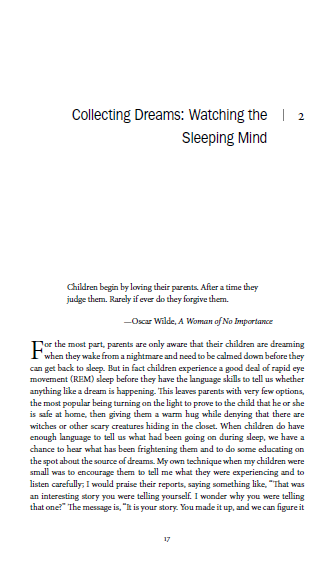
\includegraphics[width=0.48\textwidth]{./chapters/chapter49}\hfill
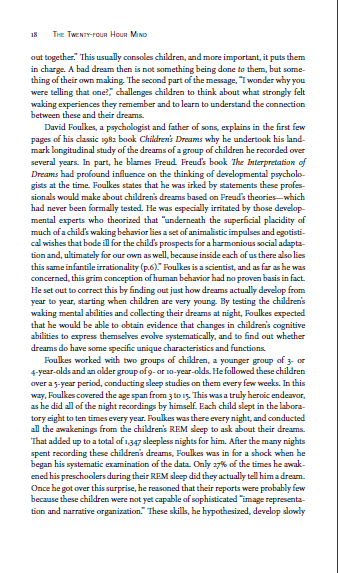
\includegraphics[width=0.48\textwidth]{./chapters/chapter49a}
\caption{Style 49 from the Oxford Handbook of Cuneiform Culture.}
\end{figure}
